%-*-latex-*-
\tinysidebar{\debug{exercises/{introduction-to-group-theory-2/answer.tex}}}

(a) In $S_5$,
\begin{align*}
\left( (1 \ 4 \ 3)(2 \ 5) \circ (2 \ 3 \ 5) \right)(1) = \left( (1 \ 4 \ 3)(2 \ 5)\right)(1) &= 4 \\
\left( (1 \ 4 \ 3)(2 \ 5) \circ (2 \ 3 \ 5) \right)(2) = \left( (1 \ 4 \ 3)(2 \ 5)\right)(3) &= 1 \\
\left( (1 \ 4 \ 3)(2 \ 5) \circ (2 \ 3 \ 5) \right)(3) = \left( (1 \ 4 \ 3)(2 \ 5)\right)(5) &= 2 \\
\left( (1 \ 4 \ 3)(2 \ 5) \circ (2 \ 3 \ 5) \right)(4) = \left( (1 \ 4 \ 3)(2 \ 5)\right)(4) &= 3 \\
\left( (1 \ 4 \ 3)(2 \ 5) \circ (2 \ 3 \ 5) \right)(5) = \left( (1 \ 4 \ 3)(2 \ 5)\right)(2) &= 5 
\end{align*}
i.e.,
\[
(1 \ 4 \ 3)(2 \ 5) \circ (2 \ 3 \ 5) = (1 \ 4 \ 3 \ 2)(5) = (1 \ 4 \ 3 \ 2) 
\]

(b)
There are $3! = 6$ elements in $S_3$.
The permutation of $S_3$ are
\[
(1), (1 \ \ 2), (1 \ \ 3), (2 \ \ 3),
(1 \ \  2 \ \ 3),
(1 \ \  3 \ \ 2)
\]
The group table of $S_3$ is
%-*-latex-*-
\begin{center}
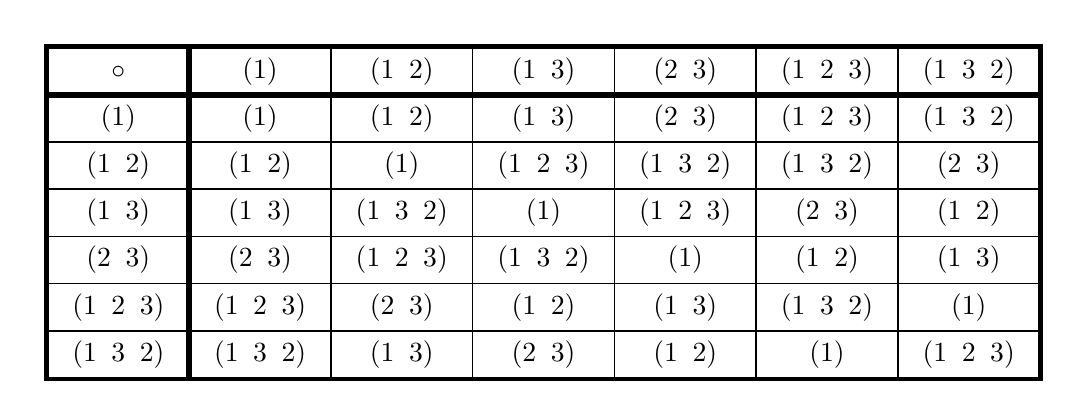
\begin{tikzpicture}

\draw (0.9, -0.3)
  node[draw, line width=0.02cm, , color=black,
       rounded corners=0cm, inner sep=0cm] {

\begin{minipage}[t][0.6cm]{1.8cm}
\mbox{}

\end{minipage}

};\draw (0.9, -0.3) node[color=black] {{\texttt{{\vphantom{$\circ$$(1)$$(1 \ 2)$$(1 \ 3)$$(2 \ 3)$$(1 \ 2 \ 3)$$(1 \ 3 \ 2)$}$\circ$}}}};\node[anchor=south] at (0.9,0.01) {};\node[anchor=east] at (-0.01,-0.3) {};
\draw (0.9, -0.3)
  node[draw, line width=0.06cm, , color=black,
       rounded corners=0cm, inner sep=0cm] {

\begin{minipage}[t][0.62cm]{1.82cm}
\mbox{}

\end{minipage}

};
\draw (2.7, -0.3)
  node[draw, line width=0.02cm, , color=black,
       rounded corners=0cm, inner sep=0cm] {

\begin{minipage}[t][0.6cm]{1.8cm}
\mbox{}

\end{minipage}

};\draw (2.7, -0.3) node[color=black] {{\texttt{{\vphantom{$\circ$$(1)$$(1 \ 2)$$(1 \ 3)$$(2 \ 3)$$(1 \ 2 \ 3)$$(1 \ 3 \ 2)$}$(1)$}}}};
\draw (4.5, -0.3)
  node[draw, line width=0.02cm, , color=black,
       rounded corners=0cm, inner sep=0cm] {

\begin{minipage}[t][0.6cm]{1.8cm}
\mbox{}

\end{minipage}

};\draw (4.5, -0.3) node[color=black] {{\texttt{{\vphantom{$\circ$$(1)$$(1 \ 2)$$(1 \ 3)$$(2 \ 3)$$(1 \ 2 \ 3)$$(1 \ 3 \ 2)$}$(1 \ 2)$}}}};
\draw (6.300000000000001, -0.3)
  node[draw, line width=0.02cm, , color=black,
       rounded corners=0cm, inner sep=0cm] {

\begin{minipage}[t][0.6cm]{1.8cm}
\mbox{}

\end{minipage}

};\draw (6.300000000000001, -0.3) node[color=black] {{\texttt{{\vphantom{$\circ$$(1)$$(1 \ 2)$$(1 \ 3)$$(2 \ 3)$$(1 \ 2 \ 3)$$(1 \ 3 \ 2)$}$(1 \ 3)$}}}};
\draw (8.100000000000001, -0.3)
  node[draw, line width=0.02cm, , color=black,
       rounded corners=0cm, inner sep=0cm] {

\begin{minipage}[t][0.6cm]{1.8cm}
\mbox{}

\end{minipage}

};\draw (8.100000000000001, -0.3) node[color=black] {{\texttt{{\vphantom{$\circ$$(1)$$(1 \ 2)$$(1 \ 3)$$(2 \ 3)$$(1 \ 2 \ 3)$$(1 \ 3 \ 2)$}$(2 \ 3)$}}}};
\draw (9.9, -0.3)
  node[draw, line width=0.02cm, , color=black,
       rounded corners=0cm, inner sep=0cm] {

\begin{minipage}[t][0.6cm]{1.8cm}
\mbox{}

\end{minipage}

};\draw (9.9, -0.3) node[color=black] {{\texttt{{\vphantom{$\circ$$(1)$$(1 \ 2)$$(1 \ 3)$$(2 \ 3)$$(1 \ 2 \ 3)$$(1 \ 3 \ 2)$}$(1 \ 2 \ 3)$}}}};
\draw (11.700000000000001, -0.3)
  node[draw, line width=0.02cm, , color=black,
       rounded corners=0cm, inner sep=0cm] {

\begin{minipage}[t][0.6cm]{1.8cm}
\mbox{}

\end{minipage}

};\draw (11.700000000000001, -0.3) node[color=black] {{\texttt{{\vphantom{$\circ$$(1)$$(1 \ 2)$$(1 \ 3)$$(2 \ 3)$$(1 \ 2 \ 3)$$(1 \ 3 \ 2)$}$(1 \ 3 \ 2)$}}}};\node[anchor=south] at (2.7,0.01) {};\node[anchor=south] at (4.5,0.01) {};\node[anchor=south] at (6.300000000000001,0.01) {};\node[anchor=south] at (8.100000000000001,0.01) {};\node[anchor=south] at (9.9,0.01) {};\node[anchor=south] at (11.700000000000001,0.01) {};\node[anchor=east] at (1.79,-0.3) {};
\draw (7.2, -0.3)
  node[draw, line width=0.06cm, , color=black,
       rounded corners=0cm, inner sep=0cm] {

\begin{minipage}[t][0.62cm]{10.82cm}
\mbox{}

\end{minipage}

};
\draw (0.9, -0.8999999999999999)
  node[draw, line width=0.02cm, , color=black,
       rounded corners=0cm, inner sep=0cm] {

\begin{minipage}[t][0.6cm]{1.8cm}
\mbox{}

\end{minipage}

};\draw (0.9, -0.8999999999999999) node[color=black] {{\texttt{{\vphantom{$\circ$$(1)$$(1 \ 2)$$(1 \ 3)$$(2 \ 3)$$(1 \ 2 \ 3)$$(1 \ 3 \ 2)$}$(1)$}}}};
\draw (0.9, -1.4999999999999998)
  node[draw, line width=0.02cm, , color=black,
       rounded corners=0cm, inner sep=0cm] {

\begin{minipage}[t][0.6cm]{1.8cm}
\mbox{}

\end{minipage}

};\draw (0.9, -1.4999999999999998) node[color=black] {{\texttt{{\vphantom{$\circ$$(1)$$(1 \ 2)$$(1 \ 3)$$(2 \ 3)$$(1 \ 2 \ 3)$$(1 \ 3 \ 2)$}$(1 \ 2)$}}}};
\draw (0.9, -2.0999999999999996)
  node[draw, line width=0.02cm, , color=black,
       rounded corners=0cm, inner sep=0cm] {

\begin{minipage}[t][0.6cm]{1.8cm}
\mbox{}

\end{minipage}

};\draw (0.9, -2.0999999999999996) node[color=black] {{\texttt{{\vphantom{$\circ$$(1)$$(1 \ 2)$$(1 \ 3)$$(2 \ 3)$$(1 \ 2 \ 3)$$(1 \ 3 \ 2)$}$(1 \ 3)$}}}};
\draw (0.9, -2.7)
  node[draw, line width=0.02cm, , color=black,
       rounded corners=0cm, inner sep=0cm] {

\begin{minipage}[t][0.6cm]{1.8cm}
\mbox{}

\end{minipage}

};\draw (0.9, -2.7) node[color=black] {{\texttt{{\vphantom{$\circ$$(1)$$(1 \ 2)$$(1 \ 3)$$(2 \ 3)$$(1 \ 2 \ 3)$$(1 \ 3 \ 2)$}$(2 \ 3)$}}}};
\draw (0.9, -3.3000000000000007)
  node[draw, line width=0.02cm, , color=black,
       rounded corners=0cm, inner sep=0cm] {

\begin{minipage}[t][0.6cm]{1.8cm}
\mbox{}

\end{minipage}

};\draw (0.9, -3.3000000000000007) node[color=black] {{\texttt{{\vphantom{$\circ$$(1)$$(1 \ 2)$$(1 \ 3)$$(2 \ 3)$$(1 \ 2 \ 3)$$(1 \ 3 \ 2)$}$(1 \ 2 \ 3)$}}}};
\draw (0.9, -3.9000000000000004)
  node[draw, line width=0.02cm, , color=black,
       rounded corners=0cm, inner sep=0cm] {

\begin{minipage}[t][0.6cm]{1.8cm}
\mbox{}

\end{minipage}

};\draw (0.9, -3.9000000000000004) node[color=black] {{\texttt{{\vphantom{$\circ$$(1)$$(1 \ 2)$$(1 \ 3)$$(2 \ 3)$$(1 \ 2 \ 3)$$(1 \ 3 \ 2)$}$(1 \ 3 \ 2)$}}}};\node[anchor=south] at (0.9,-0.59) {};\node[anchor=east] at (-0.01,-0.8999999999999999) {};\node[anchor=east] at (-0.01,-1.4999999999999998) {};\node[anchor=east] at (-0.01,-2.0999999999999996) {};\node[anchor=east] at (-0.01,-2.7) {};\node[anchor=east] at (-0.01,-3.3000000000000007) {};\node[anchor=east] at (-0.01,-3.9000000000000004) {};
\draw (0.9, -2.4)
  node[draw, line width=0.06cm, , color=black,
       rounded corners=0cm, inner sep=0cm] {

\begin{minipage}[t][3.62cm]{1.82cm}
\mbox{}

\end{minipage}

};
\draw (2.7, -0.8999999999999999)
  node[draw, line width=0.02cm, , color=black,
       rounded corners=0cm, inner sep=0cm] {

\begin{minipage}[t][0.6cm]{1.8cm}
\mbox{}

\end{minipage}

};\draw (2.7, -0.8999999999999999) node[color=black] {{\texttt{{\vphantom{$\circ$$(1)$$(1 \ 2)$$(1 \ 3)$$(2 \ 3)$$(1 \ 2 \ 3)$$(1 \ 3 \ 2)$}$(1)$}}}};
\draw (4.5, -0.8999999999999999)
  node[draw, line width=0.02cm, , color=black,
       rounded corners=0cm, inner sep=0cm] {

\begin{minipage}[t][0.6cm]{1.8cm}
\mbox{}

\end{minipage}

};\draw (4.5, -0.8999999999999999) node[color=black] {{\texttt{{\vphantom{$\circ$$(1)$$(1 \ 2)$$(1 \ 3)$$(2 \ 3)$$(1 \ 2 \ 3)$$(1 \ 3 \ 2)$}$(1 \ 2)$}}}};
\draw (6.300000000000001, -0.8999999999999999)
  node[draw, line width=0.02cm, , color=black,
       rounded corners=0cm, inner sep=0cm] {

\begin{minipage}[t][0.6cm]{1.8cm}
\mbox{}

\end{minipage}

};\draw (6.300000000000001, -0.8999999999999999) node[color=black] {{\texttt{{\vphantom{$\circ$$(1)$$(1 \ 2)$$(1 \ 3)$$(2 \ 3)$$(1 \ 2 \ 3)$$(1 \ 3 \ 2)$}$(1 \ 3)$}}}};
\draw (8.100000000000001, -0.8999999999999999)
  node[draw, line width=0.02cm, , color=black,
       rounded corners=0cm, inner sep=0cm] {

\begin{minipage}[t][0.6cm]{1.8cm}
\mbox{}

\end{minipage}

};\draw (8.100000000000001, -0.8999999999999999) node[color=black] {{\texttt{{\vphantom{$\circ$$(1)$$(1 \ 2)$$(1 \ 3)$$(2 \ 3)$$(1 \ 2 \ 3)$$(1 \ 3 \ 2)$}$(2 \ 3)$}}}};
\draw (9.9, -0.8999999999999999)
  node[draw, line width=0.02cm, , color=black,
       rounded corners=0cm, inner sep=0cm] {

\begin{minipage}[t][0.6cm]{1.8cm}
\mbox{}

\end{minipage}

};\draw (9.9, -0.8999999999999999) node[color=black] {{\texttt{{\vphantom{$\circ$$(1)$$(1 \ 2)$$(1 \ 3)$$(2 \ 3)$$(1 \ 2 \ 3)$$(1 \ 3 \ 2)$}$(1 \ 2 \ 3)$}}}};
\draw (11.700000000000001, -0.8999999999999999)
  node[draw, line width=0.02cm, , color=black,
       rounded corners=0cm, inner sep=0cm] {

\begin{minipage}[t][0.6cm]{1.8cm}
\mbox{}

\end{minipage}

};\draw (11.700000000000001, -0.8999999999999999) node[color=black] {{\texttt{{\vphantom{$\circ$$(1)$$(1 \ 2)$$(1 \ 3)$$(2 \ 3)$$(1 \ 2 \ 3)$$(1 \ 3 \ 2)$}$(1 \ 3 \ 2)$}}}};
\draw (2.7, -1.4999999999999998)
  node[draw, line width=0.02cm, , color=black,
       rounded corners=0cm, inner sep=0cm] {

\begin{minipage}[t][0.6cm]{1.8cm}
\mbox{}

\end{minipage}

};\draw (2.7, -1.4999999999999998) node[color=black] {{\texttt{{\vphantom{$\circ$$(1)$$(1 \ 2)$$(1 \ 3)$$(2 \ 3)$$(1 \ 2 \ 3)$$(1 \ 3 \ 2)$}$(1 \ 2)$}}}};
\draw (4.5, -1.4999999999999998)
  node[draw, line width=0.02cm, , color=black,
       rounded corners=0cm, inner sep=0cm] {

\begin{minipage}[t][0.6cm]{1.8cm}
\mbox{}

\end{minipage}

};\draw (4.5, -1.4999999999999998) node[color=black] {{\texttt{{\vphantom{$\circ$$(1)$$(1 \ 2)$$(1 \ 3)$$(2 \ 3)$$(1 \ 2 \ 3)$$(1 \ 3 \ 2)$}$(1)$}}}};
\draw (6.300000000000001, -1.4999999999999998)
  node[draw, line width=0.02cm, , color=black,
       rounded corners=0cm, inner sep=0cm] {

\begin{minipage}[t][0.6cm]{1.8cm}
\mbox{}

\end{minipage}

};\draw (6.300000000000001, -1.4999999999999998) node[color=black] {{\texttt{{\vphantom{$\circ$$(1)$$(1 \ 2)$$(1 \ 3)$$(2 \ 3)$$(1 \ 2 \ 3)$$(1 \ 3 \ 2)$}$(1 \ 2 \ 3)$}}}};
\draw (8.100000000000001, -1.4999999999999998)
  node[draw, line width=0.02cm, , color=black,
       rounded corners=0cm, inner sep=0cm] {

\begin{minipage}[t][0.6cm]{1.8cm}
\mbox{}

\end{minipage}

};\draw (8.100000000000001, -1.4999999999999998) node[color=black] {{\texttt{{\vphantom{$\circ$$(1)$$(1 \ 2)$$(1 \ 3)$$(2 \ 3)$$(1 \ 2 \ 3)$$(1 \ 3 \ 2)$}$(1 \ 3 \ 2)$}}}};
\draw (9.9, -1.4999999999999998)
  node[draw, line width=0.02cm, , color=black,
       rounded corners=0cm, inner sep=0cm] {

\begin{minipage}[t][0.6cm]{1.8cm}
\mbox{}

\end{minipage}

};\draw (9.9, -1.4999999999999998) node[color=black] {{\texttt{{\vphantom{$\circ$$(1)$$(1 \ 2)$$(1 \ 3)$$(2 \ 3)$$(1 \ 2 \ 3)$$(1 \ 3 \ 2)$}$(1 \ 3 \ 2)$}}}};
\draw (11.700000000000001, -1.4999999999999998)
  node[draw, line width=0.02cm, , color=black,
       rounded corners=0cm, inner sep=0cm] {

\begin{minipage}[t][0.6cm]{1.8cm}
\mbox{}

\end{minipage}

};\draw (11.700000000000001, -1.4999999999999998) node[color=black] {{\texttt{{\vphantom{$\circ$$(1)$$(1 \ 2)$$(1 \ 3)$$(2 \ 3)$$(1 \ 2 \ 3)$$(1 \ 3 \ 2)$}$(2 \ 3)$}}}};
\draw (2.7, -2.0999999999999996)
  node[draw, line width=0.02cm, , color=black,
       rounded corners=0cm, inner sep=0cm] {

\begin{minipage}[t][0.6cm]{1.8cm}
\mbox{}

\end{minipage}

};\draw (2.7, -2.0999999999999996) node[color=black] {{\texttt{{\vphantom{$\circ$$(1)$$(1 \ 2)$$(1 \ 3)$$(2 \ 3)$$(1 \ 2 \ 3)$$(1 \ 3 \ 2)$}$(1 \ 3)$}}}};
\draw (4.5, -2.0999999999999996)
  node[draw, line width=0.02cm, , color=black,
       rounded corners=0cm, inner sep=0cm] {

\begin{minipage}[t][0.6cm]{1.8cm}
\mbox{}

\end{minipage}

};\draw (4.5, -2.0999999999999996) node[color=black] {{\texttt{{\vphantom{$\circ$$(1)$$(1 \ 2)$$(1 \ 3)$$(2 \ 3)$$(1 \ 2 \ 3)$$(1 \ 3 \ 2)$}$(1 \ 3 \ 2)$}}}};
\draw (6.300000000000001, -2.0999999999999996)
  node[draw, line width=0.02cm, , color=black,
       rounded corners=0cm, inner sep=0cm] {

\begin{minipage}[t][0.6cm]{1.8cm}
\mbox{}

\end{minipage}

};\draw (6.300000000000001, -2.0999999999999996) node[color=black] {{\texttt{{\vphantom{$\circ$$(1)$$(1 \ 2)$$(1 \ 3)$$(2 \ 3)$$(1 \ 2 \ 3)$$(1 \ 3 \ 2)$}$(1)$}}}};
\draw (8.100000000000001, -2.0999999999999996)
  node[draw, line width=0.02cm, , color=black,
       rounded corners=0cm, inner sep=0cm] {

\begin{minipage}[t][0.6cm]{1.8cm}
\mbox{}

\end{minipage}

};\draw (8.100000000000001, -2.0999999999999996) node[color=black] {{\texttt{{\vphantom{$\circ$$(1)$$(1 \ 2)$$(1 \ 3)$$(2 \ 3)$$(1 \ 2 \ 3)$$(1 \ 3 \ 2)$}$(1 \ 2 \ 3)$}}}};
\draw (9.9, -2.0999999999999996)
  node[draw, line width=0.02cm, , color=black,
       rounded corners=0cm, inner sep=0cm] {

\begin{minipage}[t][0.6cm]{1.8cm}
\mbox{}

\end{minipage}

};\draw (9.9, -2.0999999999999996) node[color=black] {{\texttt{{\vphantom{$\circ$$(1)$$(1 \ 2)$$(1 \ 3)$$(2 \ 3)$$(1 \ 2 \ 3)$$(1 \ 3 \ 2)$}$(2 \ 3)$}}}};
\draw (11.700000000000001, -2.0999999999999996)
  node[draw, line width=0.02cm, , color=black,
       rounded corners=0cm, inner sep=0cm] {

\begin{minipage}[t][0.6cm]{1.8cm}
\mbox{}

\end{minipage}

};\draw (11.700000000000001, -2.0999999999999996) node[color=black] {{\texttt{{\vphantom{$\circ$$(1)$$(1 \ 2)$$(1 \ 3)$$(2 \ 3)$$(1 \ 2 \ 3)$$(1 \ 3 \ 2)$}$(1 \ 2)$}}}};
\draw (2.7, -2.7)
  node[draw, line width=0.02cm, , color=black,
       rounded corners=0cm, inner sep=0cm] {

\begin{minipage}[t][0.6cm]{1.8cm}
\mbox{}

\end{minipage}

};\draw (2.7, -2.7) node[color=black] {{\texttt{{\vphantom{$\circ$$(1)$$(1 \ 2)$$(1 \ 3)$$(2 \ 3)$$(1 \ 2 \ 3)$$(1 \ 3 \ 2)$}$(2 \ 3)$}}}};
\draw (4.5, -2.7)
  node[draw, line width=0.02cm, , color=black,
       rounded corners=0cm, inner sep=0cm] {

\begin{minipage}[t][0.6cm]{1.8cm}
\mbox{}

\end{minipage}

};\draw (4.5, -2.7) node[color=black] {{\texttt{{\vphantom{$\circ$$(1)$$(1 \ 2)$$(1 \ 3)$$(2 \ 3)$$(1 \ 2 \ 3)$$(1 \ 3 \ 2)$}$(1 \ 2 \ 3)$}}}};
\draw (6.300000000000001, -2.7)
  node[draw, line width=0.02cm, , color=black,
       rounded corners=0cm, inner sep=0cm] {

\begin{minipage}[t][0.6cm]{1.8cm}
\mbox{}

\end{minipage}

};\draw (6.300000000000001, -2.7) node[color=black] {{\texttt{{\vphantom{$\circ$$(1)$$(1 \ 2)$$(1 \ 3)$$(2 \ 3)$$(1 \ 2 \ 3)$$(1 \ 3 \ 2)$}$(1 \ 3 \ 2)$}}}};
\draw (8.100000000000001, -2.7)
  node[draw, line width=0.02cm, , color=black,
       rounded corners=0cm, inner sep=0cm] {

\begin{minipage}[t][0.6cm]{1.8cm}
\mbox{}

\end{minipage}

};\draw (8.100000000000001, -2.7) node[color=black] {{\texttt{{\vphantom{$\circ$$(1)$$(1 \ 2)$$(1 \ 3)$$(2 \ 3)$$(1 \ 2 \ 3)$$(1 \ 3 \ 2)$}$(1)$}}}};
\draw (9.9, -2.7)
  node[draw, line width=0.02cm, , color=black,
       rounded corners=0cm, inner sep=0cm] {

\begin{minipage}[t][0.6cm]{1.8cm}
\mbox{}

\end{minipage}

};\draw (9.9, -2.7) node[color=black] {{\texttt{{\vphantom{$\circ$$(1)$$(1 \ 2)$$(1 \ 3)$$(2 \ 3)$$(1 \ 2 \ 3)$$(1 \ 3 \ 2)$}$(1 \ 2)$}}}};
\draw (11.700000000000001, -2.7)
  node[draw, line width=0.02cm, , color=black,
       rounded corners=0cm, inner sep=0cm] {

\begin{minipage}[t][0.6cm]{1.8cm}
\mbox{}

\end{minipage}

};\draw (11.700000000000001, -2.7) node[color=black] {{\texttt{{\vphantom{$\circ$$(1)$$(1 \ 2)$$(1 \ 3)$$(2 \ 3)$$(1 \ 2 \ 3)$$(1 \ 3 \ 2)$}$(1 \ 3)$}}}};
\draw (2.7, -3.3000000000000007)
  node[draw, line width=0.02cm, , color=black,
       rounded corners=0cm, inner sep=0cm] {

\begin{minipage}[t][0.6cm]{1.8cm}
\mbox{}

\end{minipage}

};\draw (2.7, -3.3000000000000007) node[color=black] {{\texttt{{\vphantom{$\circ$$(1)$$(1 \ 2)$$(1 \ 3)$$(2 \ 3)$$(1 \ 2 \ 3)$$(1 \ 3 \ 2)$}$(1 \ 2 \ 3)$}}}};
\draw (4.5, -3.3000000000000007)
  node[draw, line width=0.02cm, , color=black,
       rounded corners=0cm, inner sep=0cm] {

\begin{minipage}[t][0.6cm]{1.8cm}
\mbox{}

\end{minipage}

};\draw (4.5, -3.3000000000000007) node[color=black] {{\texttt{{\vphantom{$\circ$$(1)$$(1 \ 2)$$(1 \ 3)$$(2 \ 3)$$(1 \ 2 \ 3)$$(1 \ 3 \ 2)$}$(2 \ 3)$}}}};
\draw (6.300000000000001, -3.3000000000000007)
  node[draw, line width=0.02cm, , color=black,
       rounded corners=0cm, inner sep=0cm] {

\begin{minipage}[t][0.6cm]{1.8cm}
\mbox{}

\end{minipage}

};\draw (6.300000000000001, -3.3000000000000007) node[color=black] {{\texttt{{\vphantom{$\circ$$(1)$$(1 \ 2)$$(1 \ 3)$$(2 \ 3)$$(1 \ 2 \ 3)$$(1 \ 3 \ 2)$}$(1 \ 2)$}}}};
\draw (8.100000000000001, -3.3000000000000007)
  node[draw, line width=0.02cm, , color=black,
       rounded corners=0cm, inner sep=0cm] {

\begin{minipage}[t][0.6cm]{1.8cm}
\mbox{}

\end{minipage}

};\draw (8.100000000000001, -3.3000000000000007) node[color=black] {{\texttt{{\vphantom{$\circ$$(1)$$(1 \ 2)$$(1 \ 3)$$(2 \ 3)$$(1 \ 2 \ 3)$$(1 \ 3 \ 2)$}$(1 \ 3)$}}}};
\draw (9.9, -3.3000000000000007)
  node[draw, line width=0.02cm, , color=black,
       rounded corners=0cm, inner sep=0cm] {

\begin{minipage}[t][0.6cm]{1.8cm}
\mbox{}

\end{minipage}

};\draw (9.9, -3.3000000000000007) node[color=black] {{\texttt{{\vphantom{$\circ$$(1)$$(1 \ 2)$$(1 \ 3)$$(2 \ 3)$$(1 \ 2 \ 3)$$(1 \ 3 \ 2)$}$(1 \ 3 \ 2)$}}}};
\draw (11.700000000000001, -3.3000000000000007)
  node[draw, line width=0.02cm, , color=black,
       rounded corners=0cm, inner sep=0cm] {

\begin{minipage}[t][0.6cm]{1.8cm}
\mbox{}

\end{minipage}

};\draw (11.700000000000001, -3.3000000000000007) node[color=black] {{\texttt{{\vphantom{$\circ$$(1)$$(1 \ 2)$$(1 \ 3)$$(2 \ 3)$$(1 \ 2 \ 3)$$(1 \ 3 \ 2)$}$(1)$}}}};
\draw (2.7, -3.9000000000000004)
  node[draw, line width=0.02cm, , color=black,
       rounded corners=0cm, inner sep=0cm] {

\begin{minipage}[t][0.6cm]{1.8cm}
\mbox{}

\end{minipage}

};\draw (2.7, -3.9000000000000004) node[color=black] {{\texttt{{\vphantom{$\circ$$(1)$$(1 \ 2)$$(1 \ 3)$$(2 \ 3)$$(1 \ 2 \ 3)$$(1 \ 3 \ 2)$}$(1 \ 3 \ 2)$}}}};
\draw (4.5, -3.9000000000000004)
  node[draw, line width=0.02cm, , color=black,
       rounded corners=0cm, inner sep=0cm] {

\begin{minipage}[t][0.6cm]{1.8cm}
\mbox{}

\end{minipage}

};\draw (4.5, -3.9000000000000004) node[color=black] {{\texttt{{\vphantom{$\circ$$(1)$$(1 \ 2)$$(1 \ 3)$$(2 \ 3)$$(1 \ 2 \ 3)$$(1 \ 3 \ 2)$}$(1 \ 3)$}}}};
\draw (6.300000000000001, -3.9000000000000004)
  node[draw, line width=0.02cm, , color=black,
       rounded corners=0cm, inner sep=0cm] {

\begin{minipage}[t][0.6cm]{1.8cm}
\mbox{}

\end{minipage}

};\draw (6.300000000000001, -3.9000000000000004) node[color=black] {{\texttt{{\vphantom{$\circ$$(1)$$(1 \ 2)$$(1 \ 3)$$(2 \ 3)$$(1 \ 2 \ 3)$$(1 \ 3 \ 2)$}$(2 \ 3)$}}}};
\draw (8.100000000000001, -3.9000000000000004)
  node[draw, line width=0.02cm, , color=black,
       rounded corners=0cm, inner sep=0cm] {

\begin{minipage}[t][0.6cm]{1.8cm}
\mbox{}

\end{minipage}

};\draw (8.100000000000001, -3.9000000000000004) node[color=black] {{\texttt{{\vphantom{$\circ$$(1)$$(1 \ 2)$$(1 \ 3)$$(2 \ 3)$$(1 \ 2 \ 3)$$(1 \ 3 \ 2)$}$(1 \ 2)$}}}};
\draw (9.9, -3.9000000000000004)
  node[draw, line width=0.02cm, , color=black,
       rounded corners=0cm, inner sep=0cm] {

\begin{minipage}[t][0.6cm]{1.8cm}
\mbox{}

\end{minipage}

};\draw (9.9, -3.9000000000000004) node[color=black] {{\texttt{{\vphantom{$\circ$$(1)$$(1 \ 2)$$(1 \ 3)$$(2 \ 3)$$(1 \ 2 \ 3)$$(1 \ 3 \ 2)$}$(1)$}}}};
\draw (11.700000000000001, -3.9000000000000004)
  node[draw, line width=0.02cm, , color=black,
       rounded corners=0cm, inner sep=0cm] {

\begin{minipage}[t][0.6cm]{1.8cm}
\mbox{}

\end{minipage}

};\draw (11.700000000000001, -3.9000000000000004) node[color=black] {{\texttt{{\vphantom{$\circ$$(1)$$(1 \ 2)$$(1 \ 3)$$(2 \ 3)$$(1 \ 2 \ 3)$$(1 \ 3 \ 2)$}$(1 \ 2 \ 3)$}}}};\node[anchor=south] at (2.7,-0.59) {};\node[anchor=south] at (4.5,-0.59) {};\node[anchor=south] at (6.300000000000001,-0.59) {};\node[anchor=south] at (8.100000000000001,-0.59) {};\node[anchor=south] at (9.9,-0.59) {};\node[anchor=south] at (11.700000000000001,-0.59) {};\node[anchor=east] at (1.79,-0.8999999999999999) {};\node[anchor=east] at (1.79,-1.4999999999999998) {};\node[anchor=east] at (1.79,-2.0999999999999996) {};\node[anchor=east] at (1.79,-2.7) {};\node[anchor=east] at (1.79,-3.3000000000000007) {};\node[anchor=east] at (1.79,-3.9000000000000004) {};
\draw (7.2, -2.4)
  node[draw, line width=0.06cm, , color=black,
       rounded corners=0cm, inner sep=0cm] {

\begin{minipage}[t][3.62cm]{10.82cm}
\mbox{}

\end{minipage}

};
\end{tikzpicture}

\end{center}



(c) From the group table, when I look at the entry at row 2, column 1
and the entry at row 1, column 2, I see two different values.
(For me, the row and column indices begin with $0$ and not $1$).
\begin{align*}
\text{row 2, column 1} &: (1 \ 2) \circ (1 \ 3) = (1 \ 3 \ 2) \\
\text{row 1, column 2} &: (1 \ 3) \circ (1 \ 2) = (1 \ 2 \ 3) 
\end{align*}
Therefore $S_3$ is non-abelian.
\qed
